\chapter{Prestazioni dei sistemi numerici}

\begin{figure}[h]
    \centering
    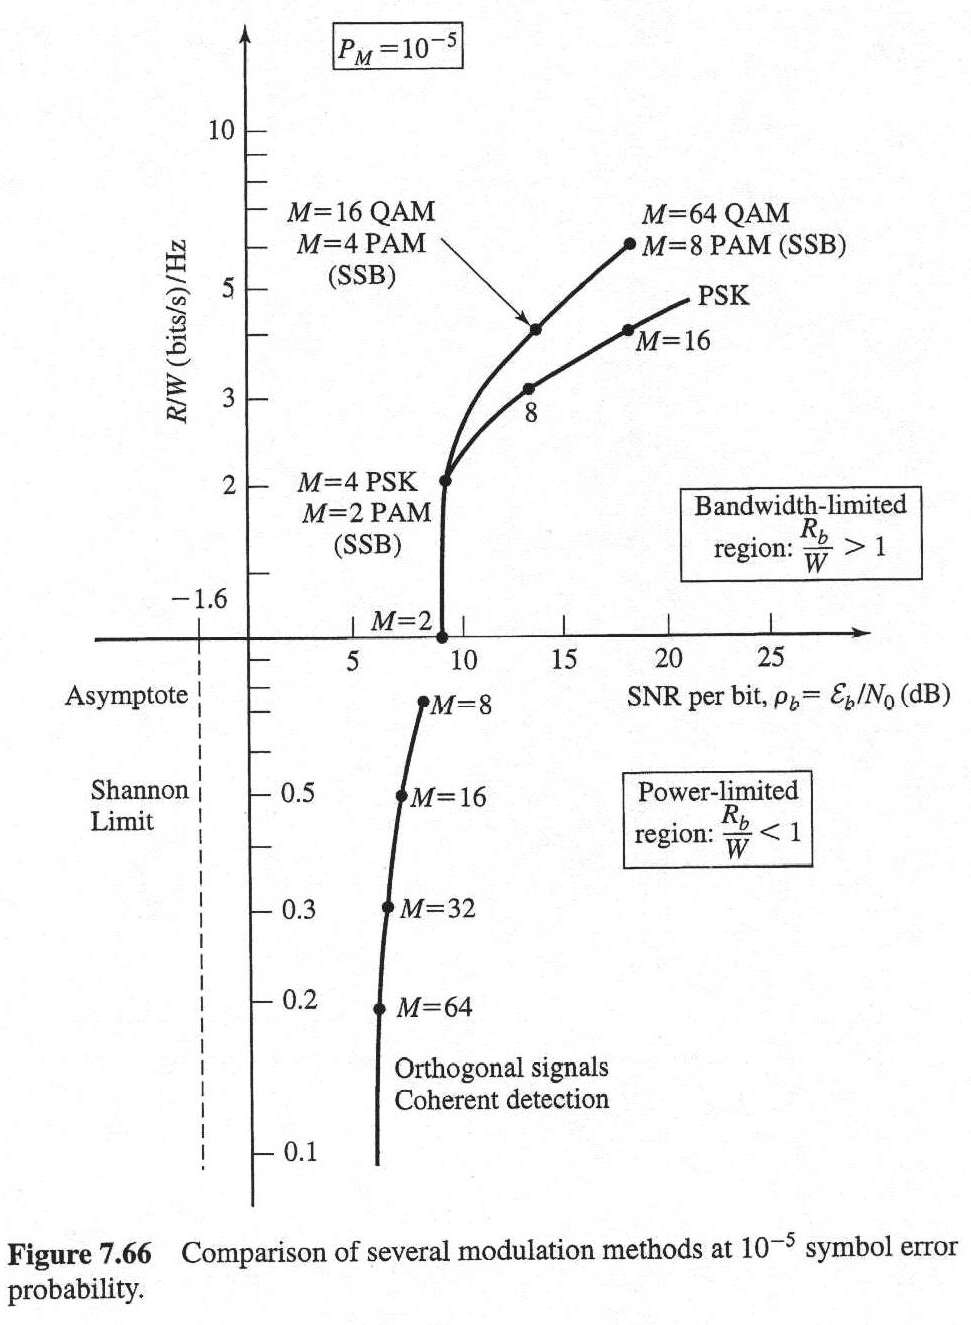
\includegraphics[scale = 0.5]{Camparare le varie modulazioni.png}
\end{figure}

\newpage 

\begin{tcolorbox}
    Questo capitolo sarà un capito pieno di formule che non dovete imparare a memoria (in caso userete queste formule per l'esercizio scritto). \newline 

    Per l'orale, 
    l'importante sono le considerazioni finali e sul perchè abbiamo tratto quelle conclusioni.  
\end{tcolorbox}

\section{Probabilità di errore per formati antipodali}
\footnote{Slide del prof | Prestazioni sistemi numerici | pag 1 - 4\\
Appunti di Damiano | pag 4 \\
Slide | Prestazioni sistemi numerici | pag 1 - 4 \\
Appunti | 2025-04-08 | pag 2 - 4
}

Consideriamo la costellazione di un formato anti-podale, 
quindi come nella 2-PAM, 2-ASK e 2-PSK: 

\begin{figure}[h]
    \centering
    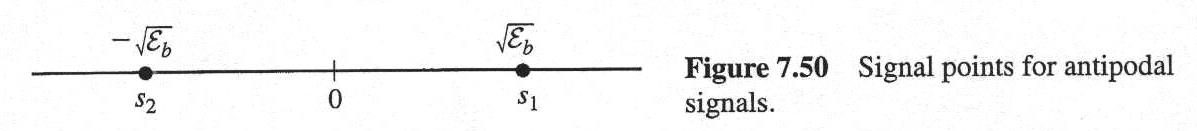
\includegraphics[scale = 0.7]{Costellazione di un formato antipodale.png}
\end{figure}

\begin{tcolorbox}
    Siccome in questi formati la dimensione dello spazio è N = 1, 
    non ci sarà la notazione vettoriale. \newline 

    La possiamo utilizzare, perchè alla fine è un vettore con N = 1. \newline 

    Per semplicità di notazione, per adesso, lasciamo tutto senza notazione vettoriale
\end{tcolorbox}

Ipotizzando che è stato trasmesso il simbolo $s_1$, 
allora possiamo dire che r segnale ricevuto è uguale a: 

{
    \Large 
    \begin{equation}
        \begin{split}
            r 
            &= 
            s_1 + n 
            \\
            &= 
            \sqrt{E_b} + n
        \end{split}
    \end{equation}
}

dove: 

\begin{itemize}
    \item $s_1$ è il segnale che dovremmo ricevere 
    \item n è il contributo di rumore 
    \item per segnali anti-podali, dai capitoli precedenti, sapevamo che vale $\sqrt{E_b}$ 
    \item $E_b$ è l'energia del bit
\end{itemize}

\newpage 

Grazie alle considerazioni svolte nel capitolo precedente, cioè che: 

\begin{itemize}
    \item ogni segnale trasmesso $s_m$ ha una PDF gaussiana 
    \item il segnale r dovrà essere confrontato con ogni simbolo della costellazione
\end{itemize}

allora, possiamo intanto graficare l'andamento delle PDF dei due simboli: 

\begin{figure}[h]
    \centering
    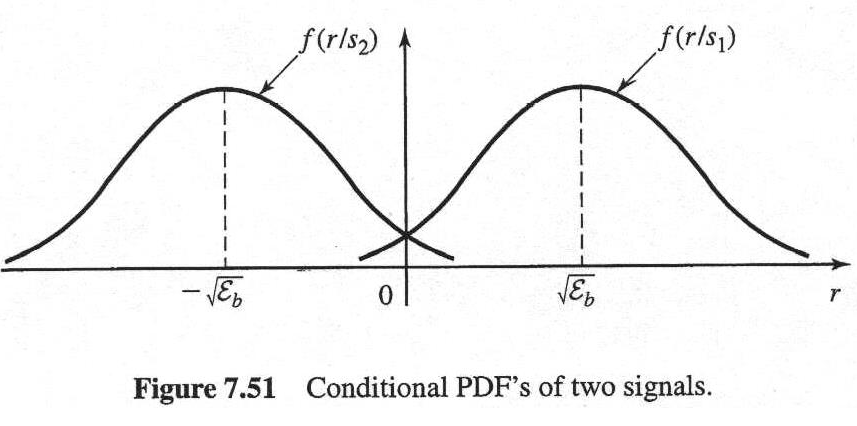
\includegraphics[scale = 0.7]{PDF di due segnali antipodali.png}
\end{figure}

e scrivere le due formule che comparano r a simboli $s_m$ della costellazione, che in questo caso sono due: 

{
    \Large 
    \begin{equation}
        f (r | s_1)
        = 
        \frac{1}{\sqrt{\pi \cdot N_0}}
        \cdot 
        \exp
        \left[
        - 
        \frac{(r - \sqrt{E_b})^{2}}{N_0}
        \right]
    \end{equation}
}

{
    \Large 
    \begin{equation}
        f (r | s_2)
        = 
        \frac{1}{\sqrt{\pi \cdot N_0}}
        \cdot 
        \exp
        \left[
        - 
        \frac{(r + \sqrt{E_b})^{2}}{N_0}
        \right]
    \end{equation}
}

Calcoliamo adesso la probabilità di errore, 
sapendo di aver trasmesso $s_1$ piuttosto che $s_2$, 
cioè ci ritroviamo r minore di 0, 
quindi nell'altra sezione di $s_2$. \newline  

Cioè in formule: 

{
    \Large 
    \begin{equation}
        \Pr {e | s_1}
        = 
        \int_{- \infty}^{0}
        f(r | s_1)
        dr
    \end{equation}
}

\begin{tcolorbox}
    Alche impostiamo l'integrale di $f(r | s_1)$ nell'intervallo $[-\infty, 0]$
\end{tcolorbox}


Facendo un po' di passi algebrici (che puoi tranquillamente ignorare perchè sono conti): 

{
    \Large 
    \begin{equation}
        \begin{split}
        \Pr {e | s_1}
        &= 
        \int_{- \infty}^{0}
        f(r | s_1)
        dr
        \\
        &= 
        \frac{1}{\sqrt{\pi \cdot N_0}}
        \cdot 
        \int_{- \infty}^{0}
        \exp 
        \left[
        - 
        \frac{(r - \sqrt{E_b})^{2}}{N_0}
        dr 
        \right]
        \\
        &= 
        \frac{1}{\sqrt{2 \pi }}
        \cdot 
        \int_{- \infty}^{- \sqrt{\frac{2 E_b}{N_0}}}
        \exp(
        - 
        \frac{x^{2}}{2}
        ) 
        dx    
        \\
        &= 
        \frac{1}{\sqrt{2 \pi }}
        \cdot 
        \int_{\sqrt{\frac{2 E_b}{N_0}}}^{\infty}
        \exp(
        - 
        \frac{x^{2}}{2}
        ) 
        dx
        \\
        &= 
        Q \left( \sqrt{\frac{2 \cdot E_b}{N_0}}\right)
        \\
        &= 
        \frac{1}{2}
        \cdot
        \text{ erfc}
        \left(
            \sqrt{\frac{E_b}{N_0}}
        \right)
        \end{split}
    \end{equation}
}

\begin{tcolorbox}

    Molto utile per lo scritto sono le tabelle erfc: le puoi visualizzare qui: \\
    \url{https://www.univpm.it/Entra/Engine/RAServeFile.php/f/P001926/allegati_ins/Erfc.pdf} \newline

    L'operatore erfc lo avevamo già studiato nel corso di Teoria dei segnali quando, appunto, stavamo 
    parlando della variabile gaussiana. \newline

    Un breve ripasso da Tds: \newline 

    \url{https://github.com/ciccio25/appunti-teoria-dei-segnali/blob/main/Appunti%20Teoria%20dei%20segnali.pdf} \\
    Capitolo 12.9.4 - Gaussiana - pag 127 - 129 

\end{tcolorbox}

Lo stesso risultato varrà anche per $s_2$: 

{
    \Large 
    \begin{equation}
        \Pr {e | s_2}
        = 
        \frac{1}{2}
        \cdot
        \text{ erfc}
        \left(
            \sqrt{\frac{E_b}{N_0}}
        \right)
    \end{equation}
}

perchè le PDF sono uguali. \newline 

Ipotizzando che i simboli sono equiprobabili, possiamo scrivere la probabilità di errore sul bit 
(cioè il bit o può valore 1 o 0, quindi o può valere $s_1$ o può valere $s_2$) e facendo qualche semplice passo algebrico: 

{
    \Large 
    \begin{equation}
        \begin{split}
            P_b
            &= 
            \frac{1}{2}
            \cdot
            \Pr(e | s_1)
            +
            \frac{1}{2}
            \cdot
            \Pr(e | s_2)
            \\
            &= 
            Q \left( \sqrt{\frac{2 \cdot E_b}{N_0}}\right)
            \\
            &=
            \frac{1}{2}
        \cdot
        \text{ erfc}
        \left(
            \sqrt{\frac{E_b}{N_0}}
        \right)
        \end{split}
    \end{equation}
}

\newpage 

Possiamo sommare le probabilità di errore di $s_1$ e $s_2$ perchè le due probabilità sono incompatibili, 
quindi indipendenti. \newline 

Nella formula di $P_b$ è presente il fattore $\frac{E_b}{N_0}$ e può essere visto come un rapporto segnale-rumore per bit. \newline 

\begin{tcolorbox}
Da ora in poi, consideriamo sempre questo rapporto cruciale per le varie trasmissioni perchè in digitale, 
rispetto all'analogico, ci interessa quanta energia E inviare dato una certa probabilità di errore. \newline 

L'argomento lo avevamo accennato nel primo capitolo di queste dispense, 
ma non ci erano noti a priori tutti gli argomenti e approfondimenti fatti fino ad adesso.
\end{tcolorbox}

Questa espressione vale per tutti i formati binari anti-podali, quindi: 
2-PAM, 2-ASK e 2-PSK. \newline 

Si considerano dei formati antipodali con canale di trasmissione di tipo BSC (in italiano Canale Binario Simmetrico), 
canale che può far variare il bit trasmesso in questa maniera: 

\begin{figure}[h]
    \centering
    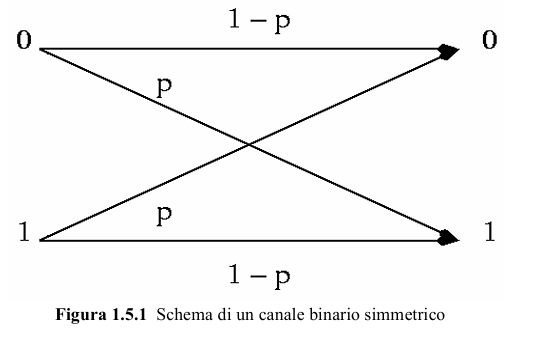
\includegraphics[scale = 0.5]{Schema canale BSC.PNG}
\end{figure}

cioè, se si trasmette uno 0, alla fine del canale, o può rimanere 0 o cambiare e diventare 1; 
stessa cosa vale se è stato trasmesso un 1. \newline 

Questa formula di $P_b$ è la migliore probabilità di errore, i.e. il gold standard, 
per un formato binario perchè è quella più piccola. \newline 

Inoltre, si considera un ricevitore coerente (e che quindi si de-modula moltiplicando il segnale modulato con una funzione sinusoidale $\cos(2 \pi f_c t)$ e filtrando nell'intorno di $f_c$) 
perchè i bit vengono inviati con la stessa energia. \newline 

All'aumentare di N, la probabilità della trasmissione peggiorerà. \newline 

\newpage 

\begin{tcolorbox}
    Oppure visto in un'altra maniera: \newline 

    
\includegraphics[scale = 0.2]{Fumetto sio.jpeg} \newline 

    \url{https://x.com/scottecs/status/1403686697938866177} \newline 

    La formula: 

    {
        \Large 
        \begin{equation}
            P_b
            = 
             \frac{1}{2}
        \cdot
        \text{ erfc}
        \left(
            \sqrt{\frac{E_b}{N_0}}
        \right)
        \end{equation}
    }

    ce la dobbiamo ricordare a memoria, proprio perchè è il gold standard.
\end{tcolorbox}

\newpage

\begin{tcolorbox}
    Non faremo i conti "carta e penna" per i prossimi formati. \newline 

    Ci dobbiamo fidare che siano veri, come i dogmi
\end{tcolorbox}

\section{Probabilità di errore per un generico formato binario con simboli equiprobabili}
\footnote{Slide del prof | Prestazioni sistemi numerici | pag 5 - 6\\
Appunti di Damiano | pag 5 - 6  \\
Slide | Prestazioni sistemi numerici | pag 5 - 6 \\
Appunti | 2025-04-08 | pag 4 - 5
}

La probabilità di errore sul bit per un generico formato binario con simboli equiprobabili vale:

{
    \Large
    \begin{equation}
        \begin{split}
            P_b 
            &= 
            Q \left( \sqrt{\frac{(d_{12})^{2}}{2 \cdot N_0}}\right)
            \\
            &= 
            \frac{1}{2}
        \cdot
        \text{ erfc}
        \left(
            \sqrt{\frac{(d_{12})^{2}}{4 \cdot N_0}}
        \right)
        \end{split}
    \end{equation}
}

dove con $d_{12}$ si indica la distanza tra due punti. \newline

Considerando come esempio i segnali ortogonali: 

\begin{figure}[h]
    \centering
    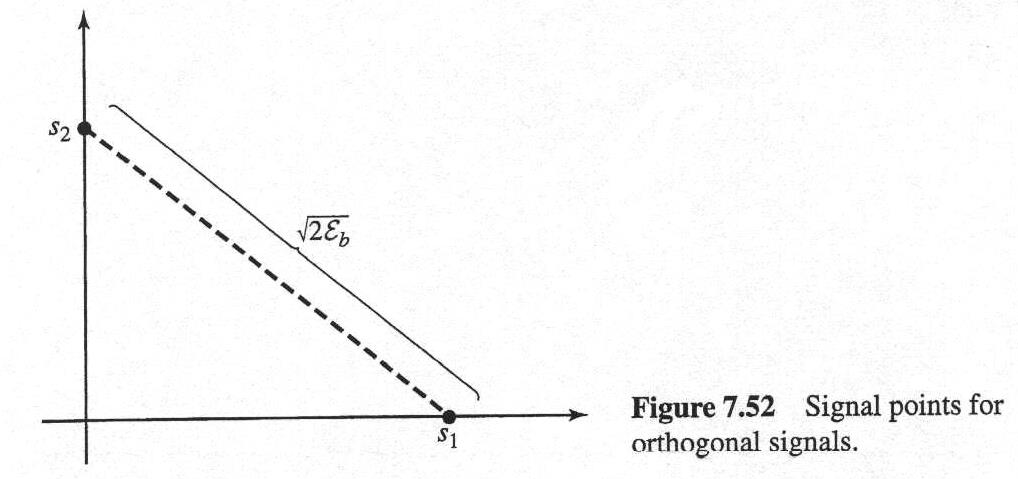
\includegraphics[scale = 0.5]{Segnali ortogoali con distanza in relazione alla energia del bit.png}
\end{figure}

Allora, la formula precedente diventa: 

{
    \Large 
    \begin{equation}
        \begin{split}
            P_b 
            &=  
            \frac{1}{2}
        \cdot
        \text{ erfc}
        \left(
            \sqrt{\frac{(d_{12})^{2}}{4 \cdot N_0}}
        \right)
        \\
        &= 
            \frac{1}{2}
        \cdot
        \text{ erfc}
        \left(
            \sqrt{\frac{(\sqrt{2 \cdot E_b})^{2}}{4 \cdot N_0}}
        \right)
        \\
        &= 
            \frac{1}{2}
        \cdot
        \text{ erfc}
        \left(
            \sqrt{\frac{2 \cdot E_b}{4 \cdot N_0}}
        \right)
        \\
        &= 
          \frac{1}{2}
        \cdot
        \text{ erfc}
        \left(
            \sqrt{\frac{E_b}{2 \cdot N_0}}
        \right)
        \end{split}
    \end{equation}
}

\begin{tcolorbox}
    Ricordiamo ancora una volta che la qualità, in una trasmissione numerica digitale, 
    non si definisce con un rapporto segnale-rumore classico, bensì tra definendo la probabilità di errore media su una finestra di misura molto ampia
\end{tcolorbox}

A parità di errore, il formato ortogonale richiede una energia doppia rispetto a quella del formato antipodale. \newline 

In dB, dovremmo aumentare la potenza di 3 dB nel formato ortogonale per avere la stessa probabilità di errore del formato antipodale. \newline 

\begin{tcolorbox}
    Questa affermazione si può dimostrare perchè se moltiplichiamo per 2 il termine sotto la radice quadra dell'erfc, quindi: 

    {
        \Large 
        \begin{equation}
            2 \cdot \frac{E_b}{2 \cdot N_0} = \frac{E_b}{N_0} 
        \end{equation}
    }

    troviamo lo stesso argomento dell'erfc, quindi la stessa probabilità di errore $P_b$ del formato anti-podale.
\end{tcolorbox}

Generalmente, piuttosto che scrivere la formula di $P_b$ e metterla in relazione con il rapporto $\frac{E_b}{N_0}$ 
si prediligono le curve come la seguente (con note): 

\begin{figure}[h]
    \centering
    \includegraphics[scale = 1]{Cuve di probabilità con note.png}
\end{figure}

Come sottolineato precedentemente, la differenza tra le curve dei due formati è proprio di 3 dB. \newline 

Generalmente queste curve vengono utilizzate per fissare la probabilità di errore $P_b$ 
(quindi fissando il valore delle ordinata), 
sapendo quale valore di $\frac{E_b}{N_0}$ utilizzare 
(quindi scegliendo di conseguenza il valore delle ascissa: in questa figura questo rapporto è indicato in dB). \newline 

\newpage 

\section{Probabilità di errore per M-PAM}
\footnote{Slide del prof | Prestazioni sistemi numerici | pag 7 - 9 \\
Appunti di Damiano | pag 8 - 9 \\
Slide | Prestazioni sistemi numerici | pag 7 - 9 \\
Appunti | 2025-04-08 | pag 5 - 6 \\
Appunti | 2025-07-21 Ricevimento | pag 8.2
}

Consideriamo la M-PAM, dove, come i casi precedenti, c'è un'unica funzione di base, quindi N = 1, 
ma rappresenteremo più segnali, quindi M sarà maggiore di 2. \newline 

Dal punto di vista grafico, possiamo visualizzare i simboli della M-PAM in una ascissa: 

\begin{figure}[h]
    \centering
    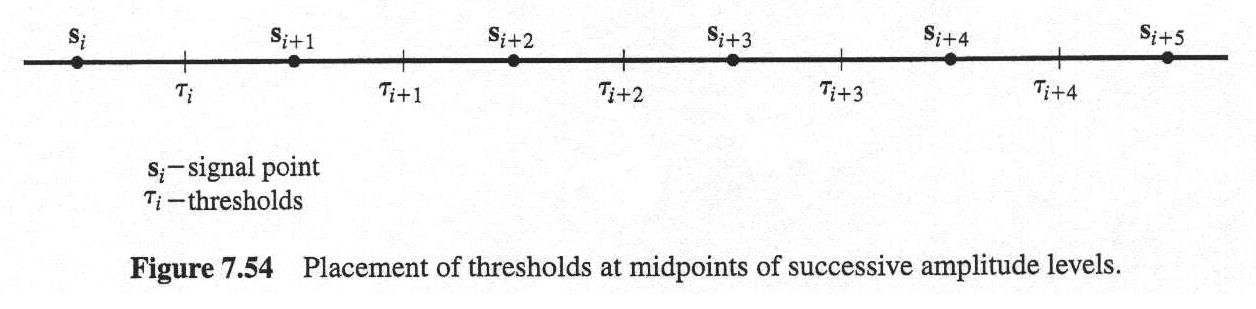
\includegraphics[scale = 0.6]{Costellazione della M-PAM.png}
\end{figure}

Come i casi precedenti, anche qui le PDF per ogni simbolo è di tipo gaussiano. \newline 

Se consideriamo le PDF di ogni simboli della M-PAM, 
potremmo vedere la figura precedente in questa maniera:

\begin{figure}[h]
    \centering
    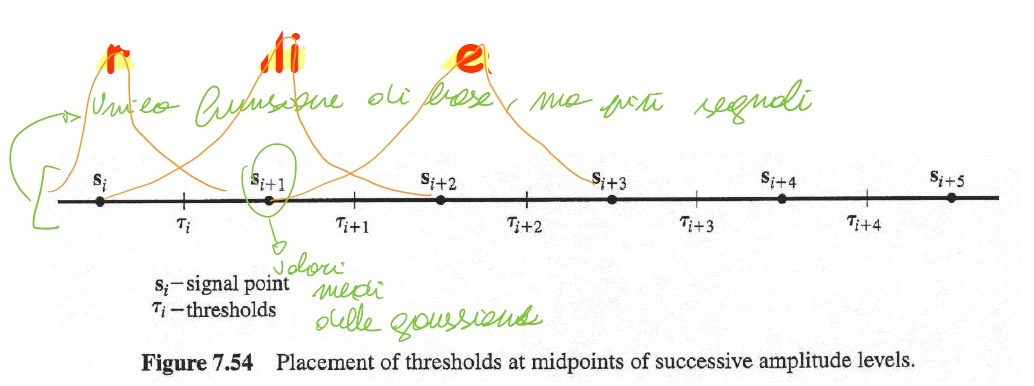
\includegraphics[scale = 0.8]{Costellazione della M-PAM con PDF gaussiane.png}
\end{figure}

Possiamo calcolare l'energia media $E_{ave}$ di tutti i segnali della M-PAM come: 

{
    \Large 
    \begin{equation}
        E_{ave}
        = 
        \frac{1}{M}
        \cdot
        \sum_{m = 1}^{M}
        E_m
    \end{equation}
}

dove $E_m$ è l'energia media di ogni simbolo di ogni gaussiana. \newline 

Facendo l'ipotesi che nella M-PAM vengano utilizzati degli impulsi rettangoli di ampiezza $\pm 1, \pm 3, \dots$, 
la potenza media della costellazione diventa: 

\begin{tcolorbox}
Siccome partiamo da segnali con M = 1 che vanno da $[-1, +1 ]$, in cui la distanza minima è 2, 
all'aumentare di M, si vuole mantenre la stessa distanza minima. \newline 

Per esempio, per M = 2, cioè per segnali che vanno da $[-3, +3]$, la distanza minima rimane 2. \newline 

Quindi, in modulo, per segnali M-PAM, si considerano impulsi con ampiezza dispari. 
\end{tcolorbox}

{
    \Large 
    \begin{equation}
        E_{ave} = \frac{M ^{2} - 1}{3} \cdot T
    \end{equation}
}

dove: 

\begin{itemize}
    \item M sono i simboli della M-PAM 
    \item T è il periodo del simbolo
\end{itemize}

La potenza media per bit $E_{b, ave}$ è: 

{
    \Large 
    \begin{equation}
        E_{b, ave}
        =
        \frac{E_{ave}}{\log_{2} (M)}
    \end{equation}
}

La probabilità di errore sull'intero segnale vale $P_M$:

{
    \Large 
    \begin{equation}
        \begin{split}
            P_M 
            &= 
            \frac{2 \cdot (M-1)}{M}
            \cdot 
            Q
            \left(
                \frac{6 \cdot \log_{2} (M) \cdot E_{b, ave}}{(M^{2} - 1) \cdot N_0}
            \right)
            \\
            &= 
            \frac{M - 1}{M}
            \cdot 
            \text{erfc}
            \left(
                \sqrt{
                \frac{3 \cdot \log_{2} (M)}{(M^{2} - 1)}
                \cdot 
                \rho_{b, ave}
                }
            \right)
        \end{split}
    \end{equation}
}

dove: 

{
    \Large 
    \begin{equation}
        \rho_{p, ave} 
        =
        \frac{E_{b, ave}}{N_0}
    \end{equation}
}

\begin{tcolorbox}
    Per noi, $ \rho_{p, ave} $ sarà il nostro SNR, rapporto segnale-rumore
\end{tcolorbox}


Applicando il Mapping di Gray (vedi 7.4.5.1 Modulazioni con costellazioni di segnali passa-banda pag 223 - 228) 
quindi che il vettore adiacente varia solo, in codifica, di un bit, 
allora la probabilità di errore sul bit $P_b$ vale: 

{
    \Large 
    \begin{equation}
        P_b 
        = 
        \frac{P_M}{\log_{2} (M)} 
    \end{equation}
}

Visualizzando graficamente la probabilità di errore del simbolo $P_M$ rispetto all'SNR sul bit in dB, 
per un qualsiasi M, $P_M$ vale (con note): 

\begin{figure}[h]
    \centering
    \includegraphics[scale = 0.7]{M-PAM Curve di probabilità con note.PNG}
\end{figure} 

Come scritto nelle note della figura, all'aumentare di M, 
peggiora $\rho_{p, ave} $ (che per noi, in digitale è il rapporto segnale rumore). \newline 

Come scritto in precedenza, idealmente si vorrebbe aumentare M per stringere la banda, 
ma ciò comporta una maggiore probabilità di errore. \newline 

\newpage

Di seguito un confronto tra le varie M-PAM e di quanti dB aumentare per avere la stessa probabilità di errore: 

\begin{figure}[h]
    \centering
    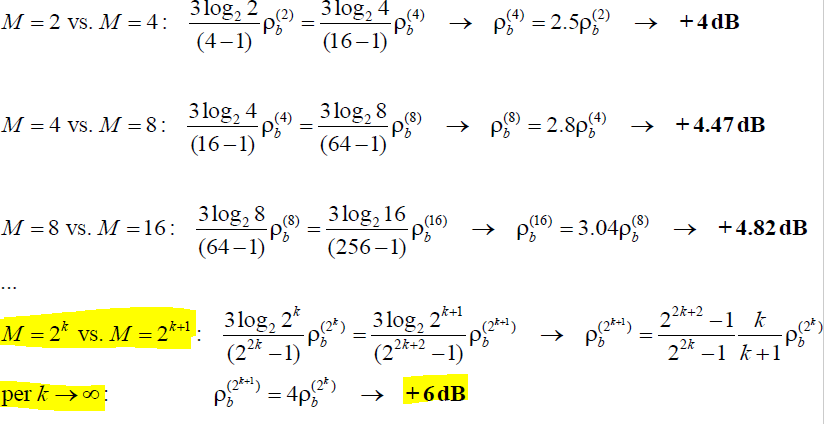
\includegraphics[scale = 1]{Confronto SNR M-PAM.PNG}
\end{figure}

Siccome consideriamo il dato peggiore, 
per M che tende ad infinito, possiamo considerare che aumentando una M-PAM 
tra una M che è una potenza di $2^{k}$ e la successiva $2^{k+1}$, 
si considera un aumento di +6 dB per mantenere lo stesso SNR, cioè bisogna aumentare in trasmissione di 4 volte l'energia. \newline 

\newpage 

\section{Probabilità di errore per M-ASK}
\footnote{Slide del prof | Prestazioni sistemi numerici | pag 10 \\
Slide | Prestazioni sistemi numerici | pag 10 \\
Appunti | 2025-04-08 | pag 6
}

Le prestazioni del formato M-ASK (probabilità di errore sul simbolo e probabilità di errore sul bit) 
sono identiche a quelle del formato M-PAM. \newline 

\begin{tcolorbox}
    Questa frase è ovvia pensando che la M-ASK è una M-PAM traslata in frequenza. 
\end{tcolorbox}

\newpage 

\section{Probabilità di errore per OOK}
\footnote{Slide del prof | Prestazioni sistemi numerici | pag 11 \\
Appunti di Damiano | pag 11  \\ 
Slide | Prestazioni sistemi numerici | pag 11 \\
Appunti | 2025-04-08 | pag 6 - 7
}

Visualizzando nel piano vettoriale i simboli dell'OOK: 

\begin{figure}[h]
    \centering
    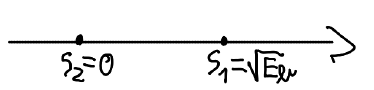
\includegraphics[scale = 0.8]{Piano vettoriale OOK.PNG}
\end{figure}

Considerando che la distanza $d_{12}$ tra due punti nella OOK vale: 

{
    \Large 
    \begin{equation}
        d_{12} = \sqrt{E_b}
    \end{equation}
}

dove con $E_b$ si considera l'energia del livello alto, cioè l'energia di piccola (perchè nella OOK si modula il segnale quando c'è il livello alto, 
invece non si manda nulla se il livello logico è basso). \newline 

Per completezza, riporto l'andamento temporale di un segnale OOK (On-Off Keying): 

\begin{figure}[h]
    \centering
    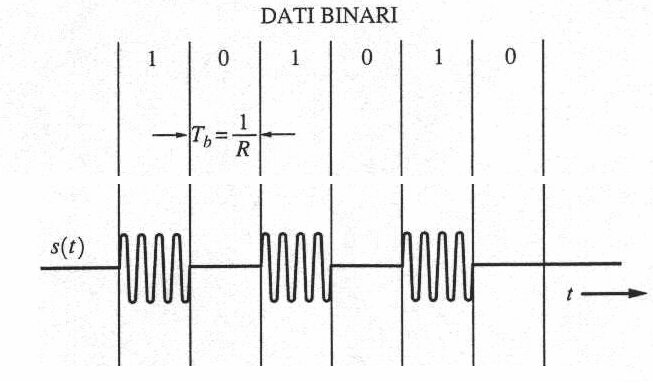
\includegraphics[scale = 0.8]{OOK andamento segnale.png}
\end{figure}

La probabilità del bit con energia di picco $P_b$ vale: 

{
    \Large 
    \begin{equation}
        \begin{split}
            P_b 
            &= 
            \frac{1}{2}
            \cdot 
            \text{erfc}
            \left(
                \sqrt{
                    \frac{(d_{12})^{2}}{4 \cdot N_0}
                }
            \right)
            \\
            &=
            \frac{1}{2}
            \cdot 
            \text{erfc}
            \left(
                \sqrt{
                    \frac{E_b}{4 \cdot N_0}
                }
            \right)
        \end{split}
    \end{equation}
}

A probabilità di errore, 
il formato OOK richiede una energia di picco 4 volte maggiore rispetto al "gold standard" della 2-ASK (in dB moltiplicare per 4 è aggiungere +6 dB). \newline 

Invece, se non si considera l'energia di picco, ma la sua media, quindi: 

{
    \Large 
    \begin{equation}
        E_{b, ave} = \frac{E_b}{2}
    \end{equation}
}

e considerando $E_{b, ave}$ l'energia media per bit, 
allora si può calcolare la probabili di errore per bit $P_b$: 

{
    \Large 
    \begin{equation}
        P_b 
        = 
        \frac{1}{2}
            \cdot 
            \text{erfc}
            \left(
                \sqrt{
                    \frac{E_{b, ave}}{2 \cdot N_0}
                }
            \right)
    \end{equation}
}

Come prima, possiamo fare la seguente considerazione. \newline 

A parità di probabilità di errore, il formato OOK richiede una energia media doppia di quella del formato 2-ASK (cioè +3 dB). \newline 

\begin{tcolorbox}
    Generalmente il rumore è più difficile gestirlo e/o diminuirlo 
    (basti pensare, come esempio, un amplificatore rumoroso, un canale rumoroso, etc. ), 
    quindi, per semplicità, si aumenta l'energia in trasmissione, in modo da avere e mantenere un SNR costante.
\end{tcolorbox}

\newpage 

\section{Probabilità di errore per M-PSK}
\footnote{Slide del prof | Prestazioni sistemi numerici | pag 12 \\
Slide | Prestazioni sistemi numerici | pag 12 \\
Appunti | 2025-04-08 | pag 7
}

La probabilità di errore sull'intero segnale in M-PSK vale circa: 

{
    \Large 
    \begin{equation}
        \begin{split}
            P_M 
            &\approx
            2 \cdot Q 
            \left(
                \sqrt{
                    2 \cdot \log_{2} (M) \cdot \sin[2](\frac{\pi}{M}) \cdot \rho_b
                }
            \right)
            \\
            &= 
            \text{erfc} 
            \left(
                \sqrt{
                    \log_{2} (M) \cdot \sin[2](\frac{\pi}{M}) \cdot \rho_b
                }
            \right)
        \end{split}
    \end{equation}
}

\begin{tcolorbox}
    Si considera circa perchè bisognerebbe svolgere un integrale doppio, 
    quindi si predilisce un'approssimazione di $P_M$
\end{tcolorbox}

dove:

{
    \Large 
    \begin{equation}
        \rho_b = \frac{E_b}{N_0}
    \end{equation}
}

Per quanto riguarda l'energia sul bit $E_b$ della M-PSK, esso vale: 

{
    \Large 
    \begin{equation}
        E_b 
        = 
        \frac{E_m}{\log_{2} (M)}
    \end{equation}
}

dove $E_m$ è l'energia media del segnale nel simbolo. \newline 

Inoltre, la probabilità di errore sul bit $P_b$ vale: 

{
    \Large 
    \begin{equation}
        P_b 
        = 
        \frac{P_M}{\log_{2} (M)}
    \end{equation}
}

Considerando il caso particolare della 2-PSK, quindi M = 2, 
$P_b$ vale: 

{
    \Large 
    \begin{equation}
        P_b 
        = 
        \frac{1}{2}
        \cdot
        \text{erfc}
        \left( \sqrt{\rho_b}\right)
    \end{equation}
}

\newpage 

\section{Probabilità di errore per DPSK}
\footnote{Slide del prof | Prestazioni sistemi numerici | pag 13 \\
Slide | Prestazioni sistemi numerici | pag 13 \\
Appunti | 2025-04-08 | pag 7 \\ 
Appunti | 2025-07-21 Ricevimento | pag 9
}

Consideriamo per adesso una rivelazione coerente per una DPSK. \newline 

L'obbiettivo è quello di eliminare il problema dell'ambiguità di fase attraverso la codifica differenziale. \newline 

La demodulazione è identica a quella della PSK, 
quindi l'errore sul bit $P_b$ vale:

{
    \Large 
    \begin{equation}
        \begin{split}
            P_b
            &= 
            \text{erfc} (\sqrt{\rho_b}) 
            \cdot 
            \left(
                1 - \frac{1}{2} \cdot \text{erfc} (\sqrt{\rho_b})
            \right)
            \\
            &\approx
            2 \cdot (P_b)_{PSK}
        \end{split}
    \end{equation}
}

Il fattore 2 è dovuto al fatto che, 
un errore nella DPSK produce di solito 2 bit errati in uscita. \newline 

Invece, se si svolge una rivelazione non coerente, $P_b$ vale: 

{
    \Large 
    \begin{equation}
        P_b = \frac{1}{2} \cdot \exp(- \rho_b)
    \end{equation}
}

Facendo i grafici di $P_b$ rispetto all'SNR sul bit e tracciando le curve della DPSK con rivelazione non coerente 
e la PSK, abbiamo il seguente andamento: 

\begin{figure}[h]
    \centering
    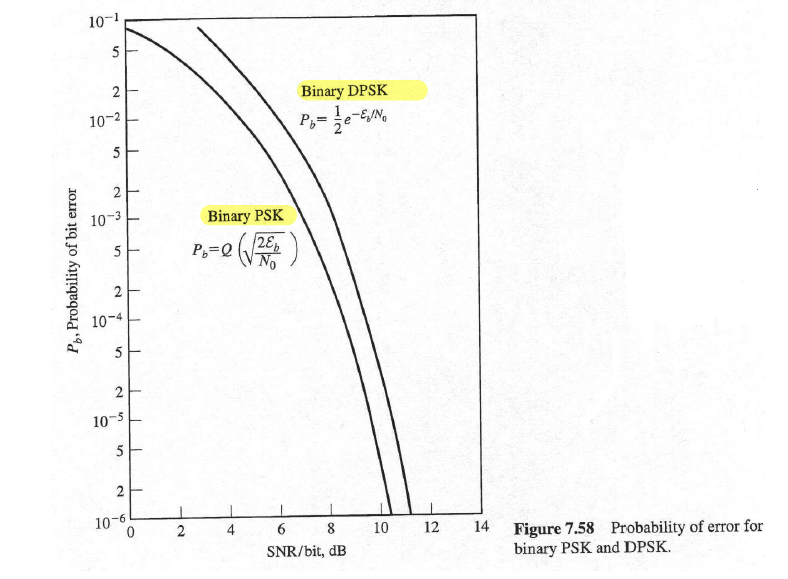
\includegraphics[scale = 1]{DPSK VS PSK.PNG}
\end{figure}

\newpage 

Quindi utilizzare la DPSK con rivelazione non coerente rispetto alla PSK si ha solo una penalizzazione di 1 dB. \newline 

\begin{tcolorbox}

Nella pagina 15 della slide ci si riferisce a, sinistra, 
una modulazione classica, invece a destra, ad una modulazione mista. \newline 

Tutte e due le modulazione hanno la stessa distanza minima. \newline 

Invece a pag 16, si considerano delle modulazioni con la stessa distanza minima, 
ma hanno energia diversa per ogni simbolo
\end{tcolorbox}

\newpage 

\section{Probabilità di errore per M-QAM}
\footnote{Slide del prof | Prestazioni sistemi numerici | pag 17 \\
Slide | Prestazioni sistemi numerici | pag 17 \\ 
Appunti | 2025-04-14 | pag 2
}

La probabilità di errore $P_M$ sull'intero segnale in M-QAM, vale: 

{
    \Large 
    \begin{equation}
        \begin{split}
            P_M 
            &\approx
            4 \cdot Q
            \left(
                \sqrt{
                    \frac{
                        3 \cdot \log_{2} (M)
                    }{M-1}
                    \cdot 
                    \rho_{b, ave}
                }
            \right)
            \\
            &= 
            2 \cdot 
            \text{erfc}
            \left(
                \sqrt{
                    \frac{
                        3 \cdot \log_{2} (M)
                    }{2 \cdot (M-1)}
                    \cdot 
                    \rho_{b, ave}
                }
            \right)
        \end{split}
    \end{equation}
}

Dalla formula di $P_M$ si può notare che, all'aumentare di M, 
$P_M$ peggiora di un fattore molto alto. \newline 

Di seguito l'andamento della probabilità di errore $P_M$ rispetto all'SNR per bit: 

\begin{figure}[h]
    \centering
    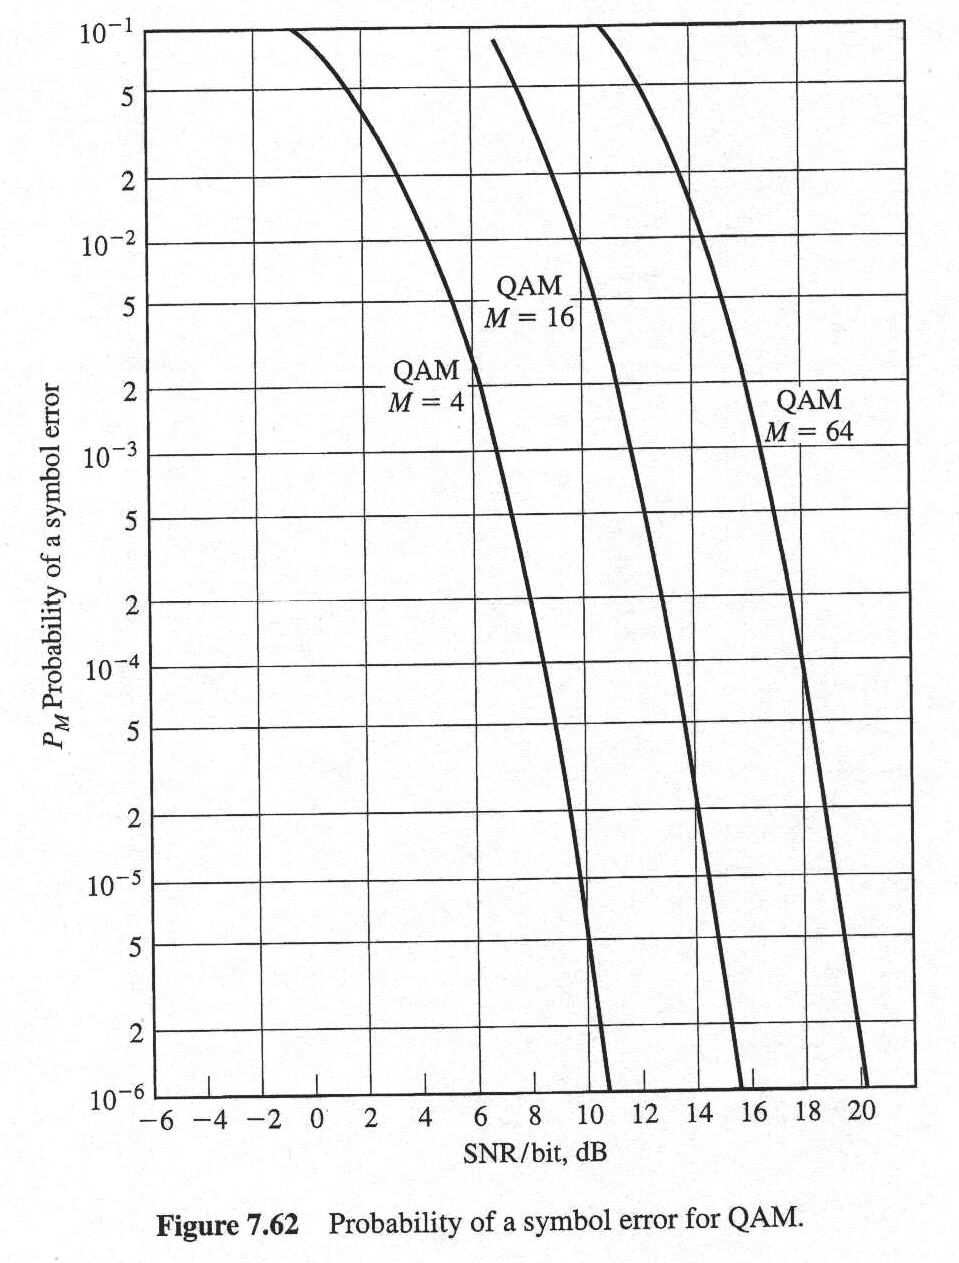
\includegraphics[scale = 0.5]{SNR QAM a confronto.png}
\end{figure}

Si considera che nella M-QAM si è applicato un mapping di Gray, quindi con k pari (in cui si avrà un quadrato perfetto della costellazione), 
invece se k è dispari, si dice che si applica un mapping quasi Gray. \newline 

Se M = 4, avremo che la 4-QAM è uguale alle 4-PSK. \newline 

\newpage 

\section{QAM vs. PSK}
\footnote{Slide del prof | Prestazioni sistemi numerici | pag 18 - 20 \\
Slide | Prestazioni sistemi numerici | pag 18 - 20 \\
Appunti | 2025-04-14 | pag 3 - 4
}

Confrontiamo le due probabilità di errore della M-QAM e della M-PSK: 

{
    \Large 
    \begin{equation}
        \left(
            P_M
        \right)_{QAM}
         \approx 
            2 \cdot 
            \text{erfc}
            \left(
                \sqrt{
                    \frac{
                        3 \cdot \log_{2} (M)
                    }{2 \cdot (M-1)}
                    \cdot 
                    \rho_{b, ave}
                }
            \right)
    \end{equation}
}

{
    \Large 
    \begin{equation}
     \left(
            P_M
        \right)_{PSK}   
      \approx 
            \text{erfc} 
            \left(
                \sqrt{
                    \log_{2} (M) \cdot \sin[2](\frac{\pi}{M}) \cdot \rho_b
                }
            \right)  
    \end{equation}
}

A livello energetico, 
la PSK ha il vincolo che tutti i segnali M devono avere la stessa energia, 
a differenza della QAM che l'energia degli M segnali può essere diversa in base alla circonferenza in cui si trova il simbolo. \newline 

QAM e PSK possono avere le stesse prestazioni, 
ma, all'aumentare di M, si predilisce utilizzare la M-QAM. \newline 

Di seguito il vantaggio analitico di usare una M-QAM rispetto a una M-PSK: 

\begin{figure}[h]
    \centering
    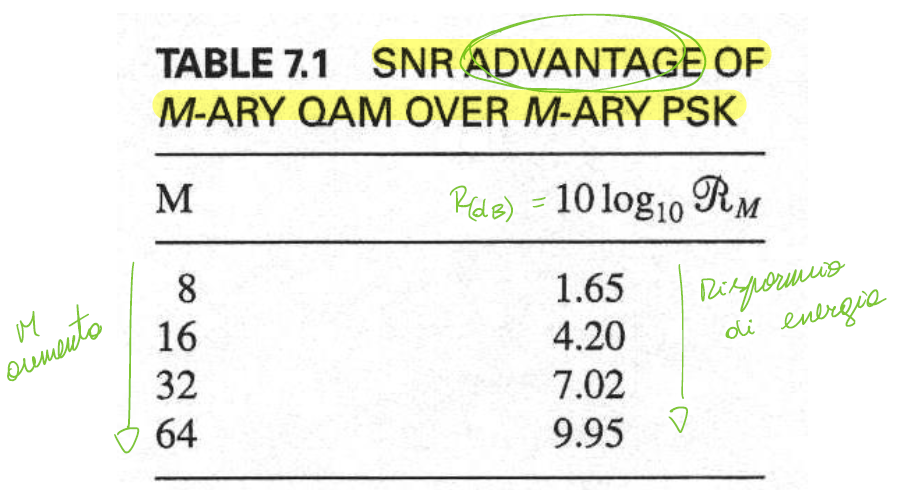
\includegraphics[scale = 0.7]{M-QAM migliore della M-PSK.PNG}
\end{figure}

Invece la seguente tabella: 

\begin{figure}[h]
    \centering
    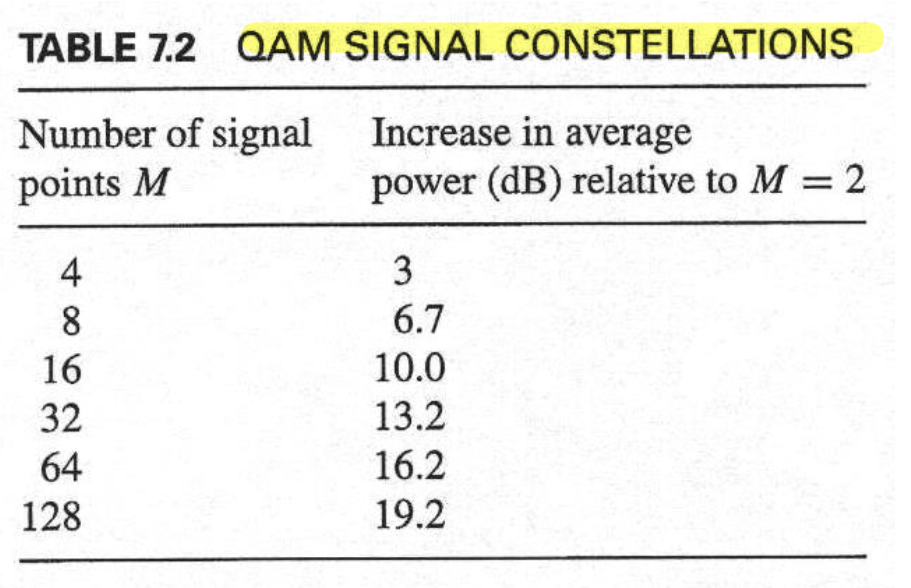
\includegraphics[scale = 0.7]{QAM aumento di potenza all'aumento di M.PNG}
\end{figure}

dimostra che, per mantenere lo stesso SNR, bisogna aumentare la potenza del segnale in trasmissione. \newline 

Quindi, siccome vogliamo aumentare M per stringere la banda, 
dobbiamo per forza aumentare la potenza in trasmissione 
per mantenere lo stesso SNR. \newline 

\newpage 

\section{Probabilità di errore formati ortogonali (ricevitore a correlatore)}
\footnote{Slide del prof | Prestazioni sistemi numerici | pag 21 \\
Slide | Prestazioni sistemi numerici | pag 21\\
Appunti | 2025-04-14 | pag 4 - 5 \\ 
Appunti | 2025-07-21 Ricevimento | pag 10
}

Considerando dei segnali equiprobabili, 
possiamo calcolare la probabilità di errore sul segnale $P_M$ utilizzando la seguente formula: 

{
    \Large 
    \begin{equation}
        P_M 
        = 
        \frac{1}{\sqrt{2 \cdot \pi}}
        \cdot 
        \int_{- \infty}^{+ \infty}
        \left\{
            1 - 
            \left[
                1 - Q(x)
            \right]^{M-1}
        \right\}
        \cdot 
        e^{- \frac{(x - \sqrt{2 \cdot \log_{2} (M) \cdot \rho_b})^{2} }{2}}
        dx
    \end{equation}
}

Invece la probabilità di errore sul bit $P_b$ vale: 

{
    \Large 
    \begin{equation}
        P_b 
        =
        \frac{2^{k - 1}}{2^{k} - 1} \cdot P_M
    \end{equation}
}

\begin{tcolorbox}

Con il simbolo k si intende $M = 2^{k}$ 

\end{tcolorbox}

Se la $P_b$ fosse uguale a 1, sarebbe il caso favorevole perchè basterebbe solo cambiare il bit: 
il problema si pone quando $P_b = \frac{1}{2}$ perchè la probabilità sta in mezzo. \newline 

Come sempre, grafichiamo l'andamento della probabilità dell'errore sul bit $P_b$ rispetto all'SNR sul bit: 

\begin{figure}[h]
    \centering
    \includegraphics[scale = 0.4]{Probabilità di errore per segnali ortogonali.png}
\end{figure}

Confrontando la figura e la formula di $P_b$, in particolare quella di $P_M$, 
notiamo che, 
all'aumentare di M, 
l'esponenziale diminuisce, 
è un decadimento molto veloce che fa tendere il fattore moltiplicativo a 1. \newline 

All'aumentare di M, l'SNR migliora per formati ortogonali con ricevitore a correlatore. \newline 

\newpage 

\subsection{Limite di Shannon}
\footnote{Slide del prof | Prestazioni sistemi numerici | pag 22 \\
Slide | Prestazioni sistemi numerici | pag 22 \\
Appunti | 2025-04-14 | pag 5
}

Il matematico Shannon ha dimostrare che, se M tende ad infinito: 

{
    \Large 
    \begin{equation}
        P_M = 0 \text{ per } \frac{E_b}{N_0} > - 1.6 \text{ dB}
    \end{equation}
}

Questa formula prende il nome di Limite di Shannon. \newline 

I formati ortogonali tendono al limite di Shannon per M che tende ad infinito. \newline 

Dal punto di vista grafico: 

\begin{figure}[h]
    \centering
    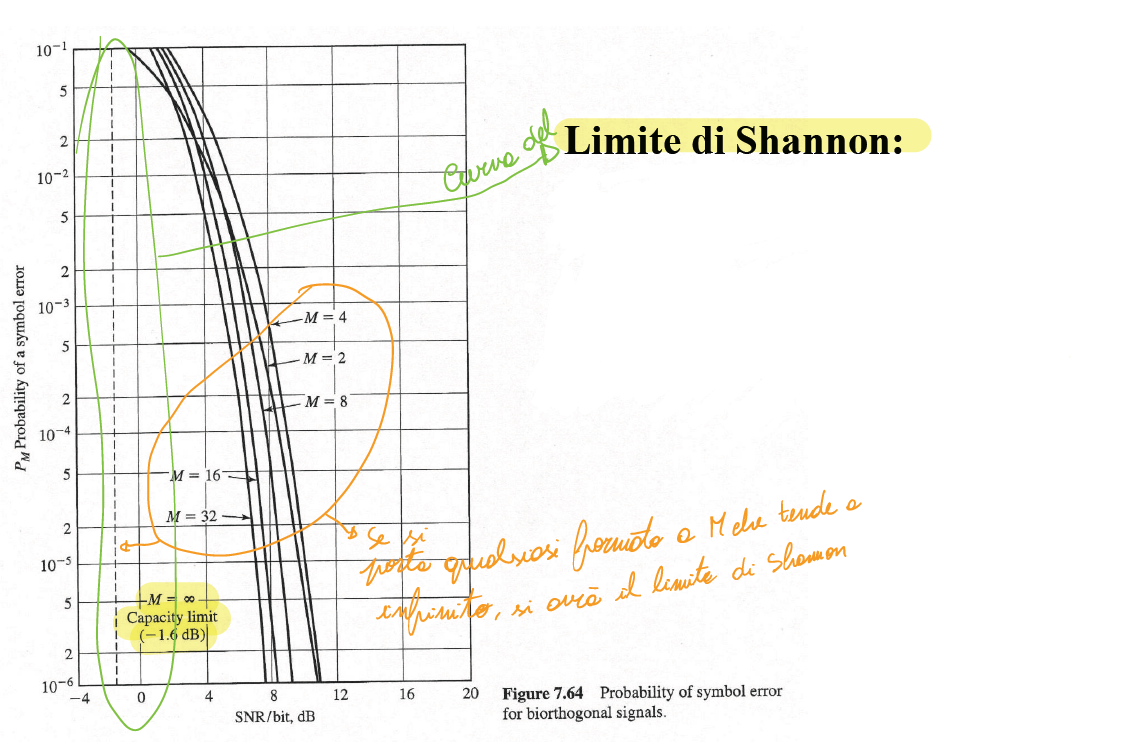
\includegraphics[scale = 0.7]{Limite di Shannon per M che tende ad infinito formati ortogonali.PNG}
\end{figure}

\newpage 

\section{Probabilità di errore formati bi-ortogonali e trans-ortogonali}
\footnote{Slide del prof | Prestazioni sistemi numerici | pag 23 \\
Slide | Prestazioni sistemi numerici | pag 23 \\
Appunti | 2025-04-14 | pag 5 - 6
}

A livello qualitativo, le probabilità di errore dei formati bi-ortogonali e trans-ortogonali sono le stesse delle ortogonali. \newline 

Di seguito le caratteristiche dei seguenti formati: 

\begin{figure}[h]
    \centering
    \includegraphics[scale = 0.7]{Probabilità di errore biortogonali e transortogonali.PNG}
\end{figure}

Per M che tende ad infinito, anche la banda del segnale tende ad infinito. \newline 

\newpage 

\section{Probabilità di errore M-FSK ortogonali (ricevitore non coerente)}
\footnote{Slide del prof | Prestazioni sistemi numerici | pag 24 \\
Slide | Prestazioni sistemi numerici | pag 24 \\
Appunti | 2025-04-14 | pag 6
}

Di seguito i dettagli della M-FSK: 

\begin{figure}[h]
    \centering
    \includegraphics[scale = 1.2]{Probabilità di errore M-FSK.PNG}
\end{figure}

\newpage 

\section{Confronto tra le modulazioni fissato una probabilità di errore sul simbolo}
\footnote{Slide del prof | Prestazioni sistemi numerici | pag 25 \\
Slide | Prestazioni sistemi numerici | pag 25 \\
Appunti | 2025-04-14 | pag 6
}

Fissato un $P_M$, con la seguente figura possiamo confrontare tutte le modulazioni studiate: 

\begin{figure}[h]
    \centering
    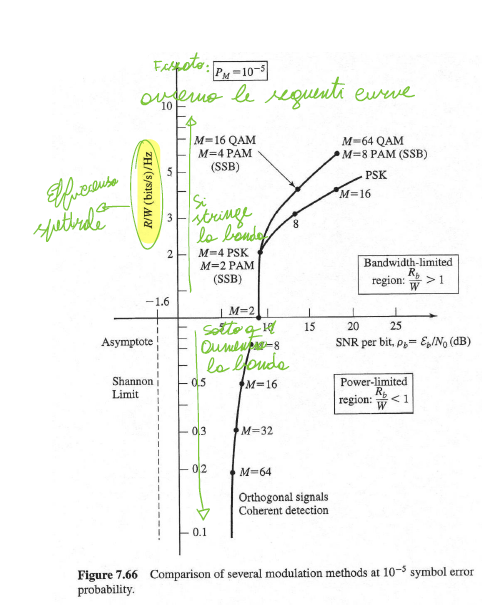
\includegraphics[scale = 1.5]{Confronto sull'SNR e le tipo di modulazioni numeriche.PNG}
\end{figure}

\newpage 
